So far, we've only worked with {\strong digital} values: driving pins \HIGH and \LOW, or (as is often the case) turning them on and off. However, the Arduino is capable of generating analog values as well---voltages somewhere in-between 0V and +5V. We use these in-between values in controlling motors or fading LEDs. In this chapter, we'll get an LED fading on and off using the Arduino's PWM (Pulse Width Modulation) features. We begin with a bit of background, however.

\section{Bouncing a (Tired) Balloon}
Imagine you have a helium balloon. Typically, if you let a helium balloon go, it floats away. However, as the balloon looses buoyancy, it approaches equilibrium, and eventually starts to be heavier than air. At this point, you can have fun ``bouncing'' the balloon upwards. That is, if you give it a bump, the balloon rises a bit, and then starts to fall again (in a kind of ``slow motion'').

PWM works in much the same way.

\newpage


\vspace{3mm}
\begin{figure}[ht]
  \begin{center}
    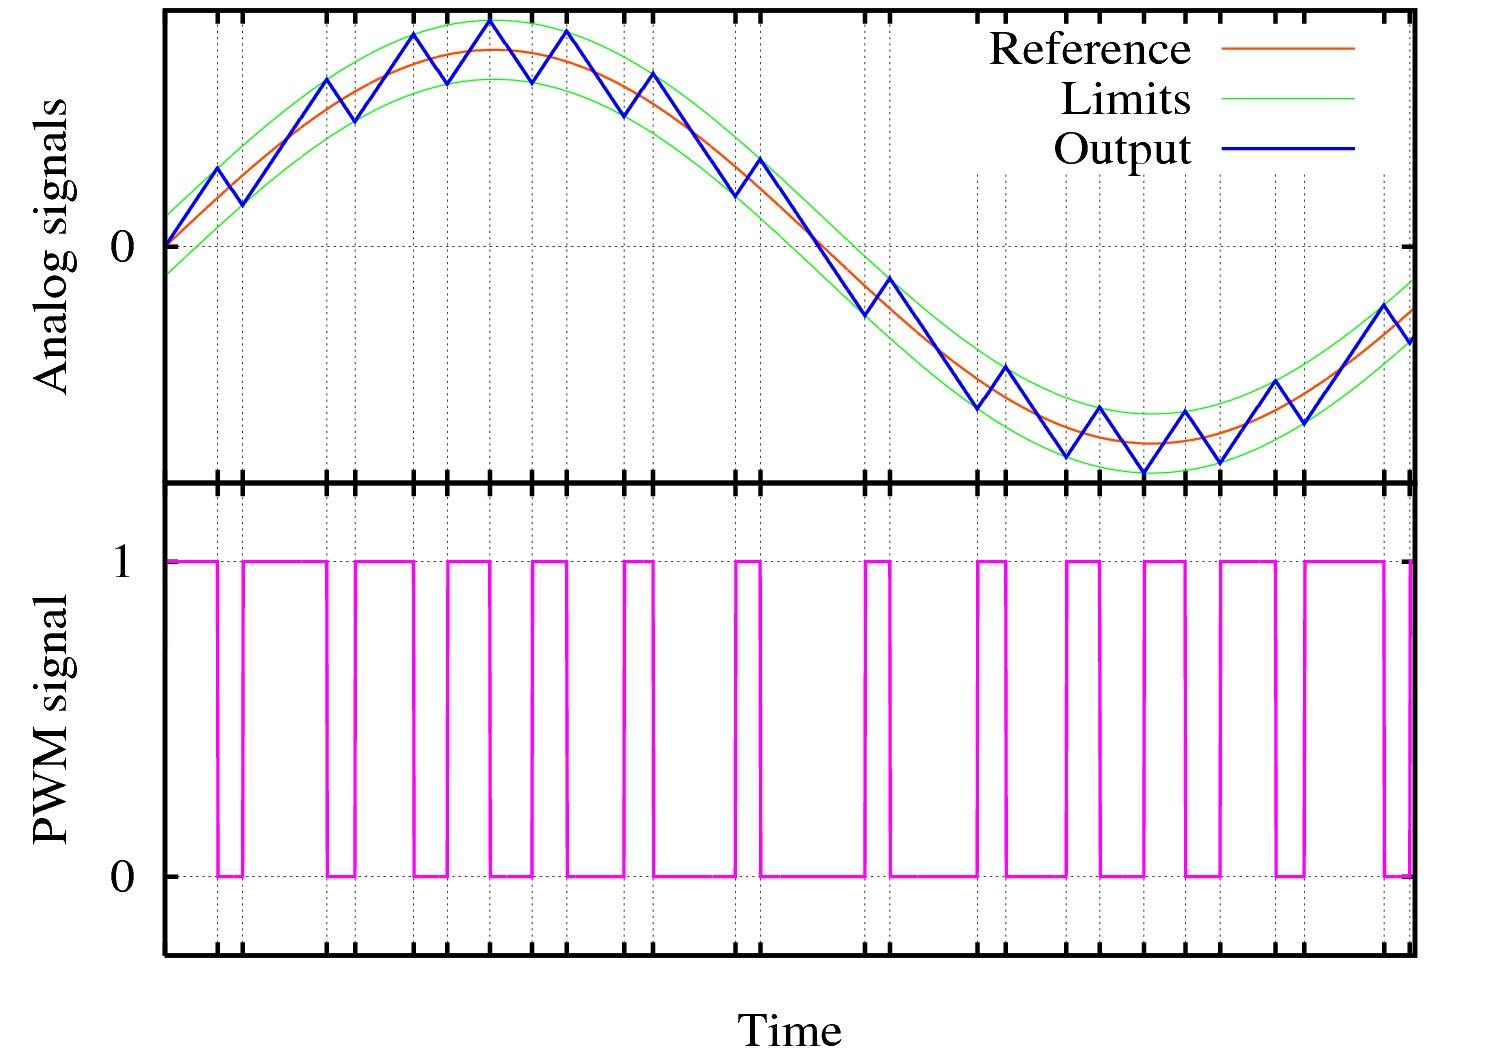
\includegraphics[width=0.9\linewidth]{images/ch7-delta-pwm}
    \caption{Delta PWM is like bouncing a balloon.}
    \label{image:ch7-delta-pwm}
  \end{center}
\end{figure}

Focus on the pink square wave in the bottom half of  Figure~\ref{image:ch7-delta-pwm}. This represents the voltage of a pin on a microcontroller like your Arduino. It starts out \HIGH, and therefore the blue line in the diagram above goes up. When the pin goes \LOW, you notice that the blue line falls. In this diagram, the blue line is your balloon; the act of ``bouncing'' the balloon is done by driving the voltage \HIGH on a pin.

Our goal is to generate an average value (the red line) by bouncing the voltage on our pin up and down (the blue line). The green lines show the points where we drive the pin \HIGH (the lower line) and the point where we stop applying voltage, or let the pin fall \LOW (the upper line). The result is that we generate, on average, the red line---our target voltage. 

\begin{comment}
We found Afrotechmod's ``PWM Tutorial'' on YouTube to be a good starting point for exploring PWM further.\footnote{ \url{http://www.youtube.com/watch?v=YmPziPfaByw}}
\end{comment}

\section{PWM on the Arduino}

Look at your Arduino:

\vspace{3mm}
\begin{figure}[ht]
  \begin{center}
    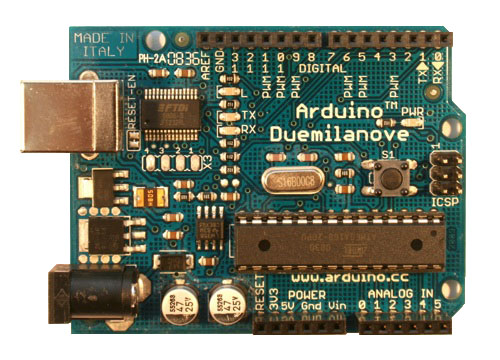
\includegraphics[width=0.9\linewidth]{images/ch7-arduino}
    \caption{PWM is available on several pins.}
    \label{image:ch7-arduino}
  \end{center}
\end{figure}

Pins 3, 5, 6, 9, 10, and 11 all have the letters {\strong PWM} underneath them. These are the only pins on your Arduino that are capable of of ``bouncing'' voltages at a very high rate of speed. If you want to fade an LED, or control a motor, you will probably be using one of these pins. It is also possible to use them as digital pins (as we have in previous chapters), but we cannot use them for both analog and digital values at the same time.

\newpage

\section{Building a Procedure}
In previous chapters we have worked with pre-existing {\PROCedure}s from the \plumbing library taken an existing \PROC apart. In this chapter, we will build one up from scratch. We'll call this \PROC {\code pwm.simple}.

\subsection{A Network Diagram}
The first thing we need to do is decide how {\code pwm.simple} will be used. While you might be accustomed to diving in and hacking code right from the start, we're going to suggest you {\em think} first. Pictures are a great way to do this.

\vspace{3mm}
\begin{figure}[ht]
  \begin{center}
    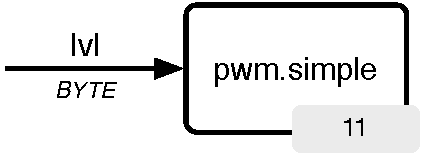
\includegraphics[width=0.8\linewidth]{images/ch7-half-network}
    \caption{Half of our process network.}
    \label{image:ch7-half-network}
  \end{center}
\end{figure}

We'll need a process that is able to change the value of a particular pin. In this example, we'll use pin \pineleven. We want other processes to be able to tell us how bright to make our LED---in a process-oriented world, data flows from one place to another over channels, so we'll have a \CHAN called {\code lvl} for that purpose. That channel can carry {\BYTE}s, or values in the range {\constant 0} to {\constant 255}.

\begin{figure*}[ht]
	\begin{center}
		{\small
		\framebox[\linewidth]{
		\begin{minipage}[t]{0.8\linewidth}

\vspace{3mm}
\subsection*{Why {\BYTE}s?}
What is a {\BYTE}, and why use it? A \BYTE is a number. The term tells us how much space is allocated in the memory of our Atmega328 (the processor on the Arduino) to store the number. A \BYTE can only be a number in the range {\constant 0} to {\constant 255}. It cannot be bigger, and it cannot be smaller. The reason for this is that 8 {\strong bits} are allocated to a \BYTE. Each bit is a zero or one (one of two possible values); this tells us that the maximum number of possible values we can represent in a \BYTE is $2^{8}$, which is {\constant 256}. Since we can represent zero, that gives us the range {\constant 0} to {\constant 255}.

\vspace{3mm}

What? That's not good enough? How about this: the Atmega328 expects, in hardware, a single byte to control the intensity of a pin. Anything more would cause problems. So we don't really have a choice: the hardware expects a byte, so we use a value of type \BYTE.
\vspace{3mm}

\end{minipage}
}}
\end{center}
\end{figure*}

At the other end of this channel we will need a process that generates numbers. We'll build that later. For now, we'll continue to focus on \pwms.

\newpage

\subsection{Choosing Parameters}
To start, we can write the shell of \PROC:

\vspace{3mm}
\begin{lstlisting}
PROC pwm.simple ( )

:
\end{lstlisting}

From our process diagram, we know that we need a constant that tells us what pin we will be using, and we need a channel that carries  {\BYTE}s. We need to put these parameters in the header of the \PROC.

\vspace{3mm}
\begin{lstlisting}
PROC pwm.simple (VAL INT pin, 
                 CHAN BYTE lvl?)

:
\end{lstlisting}
 
We say that the {\code pin} is of type \VALINT because it is a pin number (which will be an \INTeger), and we will never change this value. That is, our \PROC is not allowed to change the value of {\code pin} once we have it. By saying that {\code pin} is a \VAL, we declare it to be fixed and unchangeable.

We say the \CHANnel carries values of type \BYTE because that is what our Arduino expects us to use for representing LED intensity.

\newpage

\subsection{Just Three Steps}
Our process needs to do three things:
\begin{enumerate}
	\item Declare the pin we chose to be an {\em analog}, as opposed to {\em digital}, output pin.
	\item Read in a value from the channel.
	\item Tell the hardware to update the intensity of our LED based on the value we received.
\end{enumerate}

\subsubsection{Declaring an analog pin} 

Because we need to do these things in order, we can start by saying they will happen in \SEQuence. Remember, \occam is a fundamentally parallel programming language: when we want things to happen in lock-step, one-after-the-other, we must say \SEQ.

\vspace{3mm}
\begin{lstlisting}
PROC pwm.simple (VAL INT pin, 
                 CHAN BYTE lvl?)
  SEQ
    -- Rest of our program...
:
\end{lstlisting}

We can start by using the \plumbing procedure called \bA to declare that pin \pineleven is an analog pin. When we use \bA, that library procedure tells the Arduino to turn on PWM for the pin we choose. If we don't do this, nothing will happen when we try and set an intensity on that pin later. 

\vspace{3mm}
\begin{lstlisting}
PROC pwm.simple (VAL INT pin, 
                 CHAN BYTE lvl?)
  SEQ
    -- Enable PWM on the pin requested
    beginAnalog(pin)
:
\end{lstlisting}

\subsubsection{Reading from a \CHANnel}
To read a value, we need to do two things:
\begin{enumerate}
	\item Create a space to store what we read.
	\item Read the value from the channel.
\end{enumerate}

If a friend calls you to give you a recipe, you need paper to write it down on. That piece of paper is storage space where you can store the value (the recipe) communicated to you by your friend. Likewise, when we are reading a value from a channel, we need to create a {\strong variable} to store the value we receive. The {\strong variable} is a place to store and manipulate values.

To read a value from a channel, we use the question mark. On the {\strong left-hand side} is the name of the {\strong channel we are reading from}, and on the {\strong right-hand} side is the {\strong variable we are reading into}. The syntax for reading from a channel can be seen on the next page.

\newpage

\vspace{3mm}
\begin{figure}[ht]
  \begin{center}
    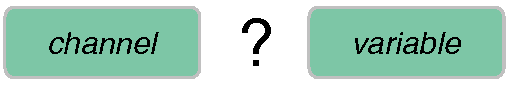
\includegraphics[width=0.8\linewidth]{images/ch7-channel-read-pattern}
    \caption{The pattern for reading from a \CHANnel.}
    \label{image:ch7-channel-read-pattern}
  \end{center}
\end{figure}

Note, though, that we first have to declare the variable that we want to read into. The syntax for declaring a variable looks like this:

\vspace{3mm}
\begin{figure}[ht]
  \begin{center}
    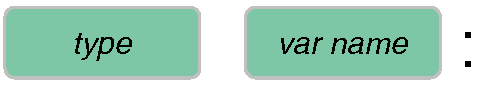
\includegraphics[width=0.8\linewidth]{images/ch7-var-decl-pattern}
    \caption{The pattern for declaring a variable.}
    \label{image:ch7-var-decl-pattern}
  \end{center}
\end{figure}

We can put these together in our program. We typically declare variables before a \SEQ, so that they can be accessed by everything within that \SEQ. We'll call this variable {\code intensity}, since it will store the intensity for our LED.

\vspace{3mm}
\begin{lstlisting}
PROC pwm.simple (VAL INT pin, 
                 CHAN BYTE lvl?)
  BYTE intensity:
  SEQ
    -- Enable PWM
    beginAnalog(pin)
    -- Read a level
    lvl ? intensity
:
\end{lstlisting}

\newpage

\subsubsection{Set the analog intensity}
We have set our pin into analog mode, we have declared space to store the level that another \PROCedure has sent to us, and we have read a value from the \CHANnel. Now, we need to use that value to change the intensity of our LED. We do this with \aW. 

\aW takes a pin number and a \BYTE---a value between {\constant 0} and {\constant 255}---and proceeds to set the pin to that intensity. If we set it to {\constant 255}, that is maximum intensity. If we set it to {\constant 127}, that is half-intensity. So, we need one more line in our \SEQ:

\vspace{3mm}
\begin{lstlisting}
PROC pwm.simple (VAL INT pin, 
                 CHAN BYTE lvl?)
  BYTE intensity:
  SEQ
    -- Enable PWM
    beginAnalog(pin)
    -- Read a level
    lvl ? intensity
    analogWrite(pin, intensity)
:
\end{lstlisting}



\newpage

\begin{comment}
\begin{lstlisting}
PROC pwm.simple (VAL INT pin, 
	               CHAN BYTE level?)
  BYTE lvl:
  SEQ
	  beginAnalog(pin)
    WHILE TRUE
      SEQ
        level ? lvl
        analogLevel(pin, lvl)
:
\end{lstlisting}
\end{comment}